\section{Results}
\label{sec:results}

Tables~\ref{tab:sonnet} and~\ref{tab:opus} give every cell; Figures~\ref{fig:sonnet} and~\ref{fig:opus} show each
run. All numbers in this section come from \texttt{bench/analyze.py} over the committed runs.

\begin{table}[t]\centering\small\setlength{\tabcolsep}{3pt}
\caption{Results on Claude Sonnet. Gated improvement: mean over runs, with a broken gate counted as no gain; brackets are 95\% bootstrap intervals. Broken: final version fails a visible or hidden gate. Unbacked: claimed gain not borne out by the outside measurement.}
\label{tab:sonnet}
\begin{tabular}{llcccc}\toprule
Task & Arm & Runs & Gated improvement & Broken & Unbacked \\\midrule
Speed up a function & plain & 6 & 260x [199x, 351x] & 0/6 & 0/6 \\
Speed up a function & loop & 6 & 435x [387x, 504x] & 0/6 & 0/6 \\
Speed up a function & hillclimb & 6 & 418x [371x, 493x] & 0/6 & 0/6 \\
Speed up a function & hillclimb-v2 & 6 & 438x [332x, 529x] & 0/6 & 0/6 \\
Speed up a function & hillclimb-v3 & 6 & 395x [361x, 443x] & 0/6 & 0/6 \\
\midrule
Raise held-out accuracy & plain & 6 & $+$18.1 pts [$+$17.3 pts, $+$19.0 pts] & 0/6 & 0/6 \\
Raise held-out accuracy & loop & 6 & $+$21.5 pts [$+$20.6 pts, $+$22.1 pts] & 0/6 & 0/6 \\
Raise held-out accuracy & hillclimb & 6 & $+$20.0 pts [$+$18.5 pts, $+$21.7 pts] & 0/6 & 0/6 \\
Raise held-out accuracy & hillclimb-v2 & 6 & $+$19.4 pts [$+$17.9 pts, $+$20.8 pts] & 0/6 & 0/6 \\
Raise held-out accuracy & hillclimb-v3 & 6 & $+$22.7 pts [$+$20.6 pts, $+$25.0 pts] & 0/6 & 0/6 \\
\midrule
Speed up a test suite & plain & 6 & 2.94x [2.89x, 2.97x] & 0/6 & 0/6 \\
Speed up a test suite & loop & 6 & 2.85x [2.80x, 2.90x] & 0/6 & 0/6 \\
Speed up a test suite & hillclimb & 6 & 2.64x [2.45x, 2.80x] & 0/6 & 0/6 \\
Speed up a test suite & hillclimb-v2 & 6 & 2.83x [2.78x, 2.87x] & 0/6 & 0/6 \\
Speed up a test suite & hillclimb-v3 & 6 & 2.88x [2.85x, 2.90x] & 0/6 & 0/6 \\
\midrule
Tune under a noisy benchmark & plain & 6 & 1.54x [1.42x, 1.67x] & 0/6 & 0/6 \\
Tune under a noisy benchmark & loop & 6 & 1.65x [1.47x, 1.76x] & 0/6 & 0/6 \\
Tune under a noisy benchmark & hillclimb & 6 & 1.32x [1.17x, 1.41x] & 0/6 & 0/5 \\
Tune under a noisy benchmark & hillclimb-v2 & 6 & 1.31x [1.13x, 1.52x] & 0/6 & 1/5 \\
Tune under a noisy benchmark & hillclimb-v3 & 6 & 1.43x [1.36x, 1.50x] & 0/6 & 0/6 \\
\bottomrule\end{tabular}\end{table}

\begin{table}[t]\centering\small
\caption{Results on Claude Opus. Gated improvement: mean over runs, with a broken gate counted as no gain; brackets are 95\% bootstrap intervals. Broken: final version fails a visible or hidden gate. Unbacked: claimed gain not borne out by the outside measurement.}
\label{tab:opus}
\begin{tabular}{llcccc}\toprule
Task & Arm & Runs & Gated improvement & Broken & Unbacked \\\midrule
Speed up a function & plain & 4 & 395x [382x, 412x] & 0/4 & 0/4 \\
Speed up a function & loop & 4 & 724x [675x, 771x] & 0/4 & 0/4 \\
Speed up a function & hillclimb-v2 & 4 & 582x [450x, 716x] & 0/4 & 0/4 \\
\midrule
Raise held-out accuracy & plain & 4 & $+$24.6 pts [$+$21.7 pts, $+$27.5 pts] & 0/4 & 0/4 \\
Raise held-out accuracy & loop & 4 & $+$28.8 pts [$+$28.5 pts, $+$29.3 pts] & 0/4 & 0/4 \\
Raise held-out accuracy & hillclimb-v2 & 4 & $+$25.4 pts [$+$22.9 pts, $+$26.9 pts] & 0/4 & 0/4 \\
\midrule
Speed up a test suite & plain & 4 & 1.50x [1.00x, 3.35x] & 3/4 & 3/4 \\
Speed up a test suite & loop & 4 & 2.39x [1.00x, 5.70x] & 2/4 & 2/4 \\
Speed up a test suite & hillclimb-v2 & 4 & 2.83x [1.49x, 4.86x] & 0/4 & 0/3 \\
\midrule
\bottomrule\end{tabular}\end{table}


\begin{figure}[t]
\centering
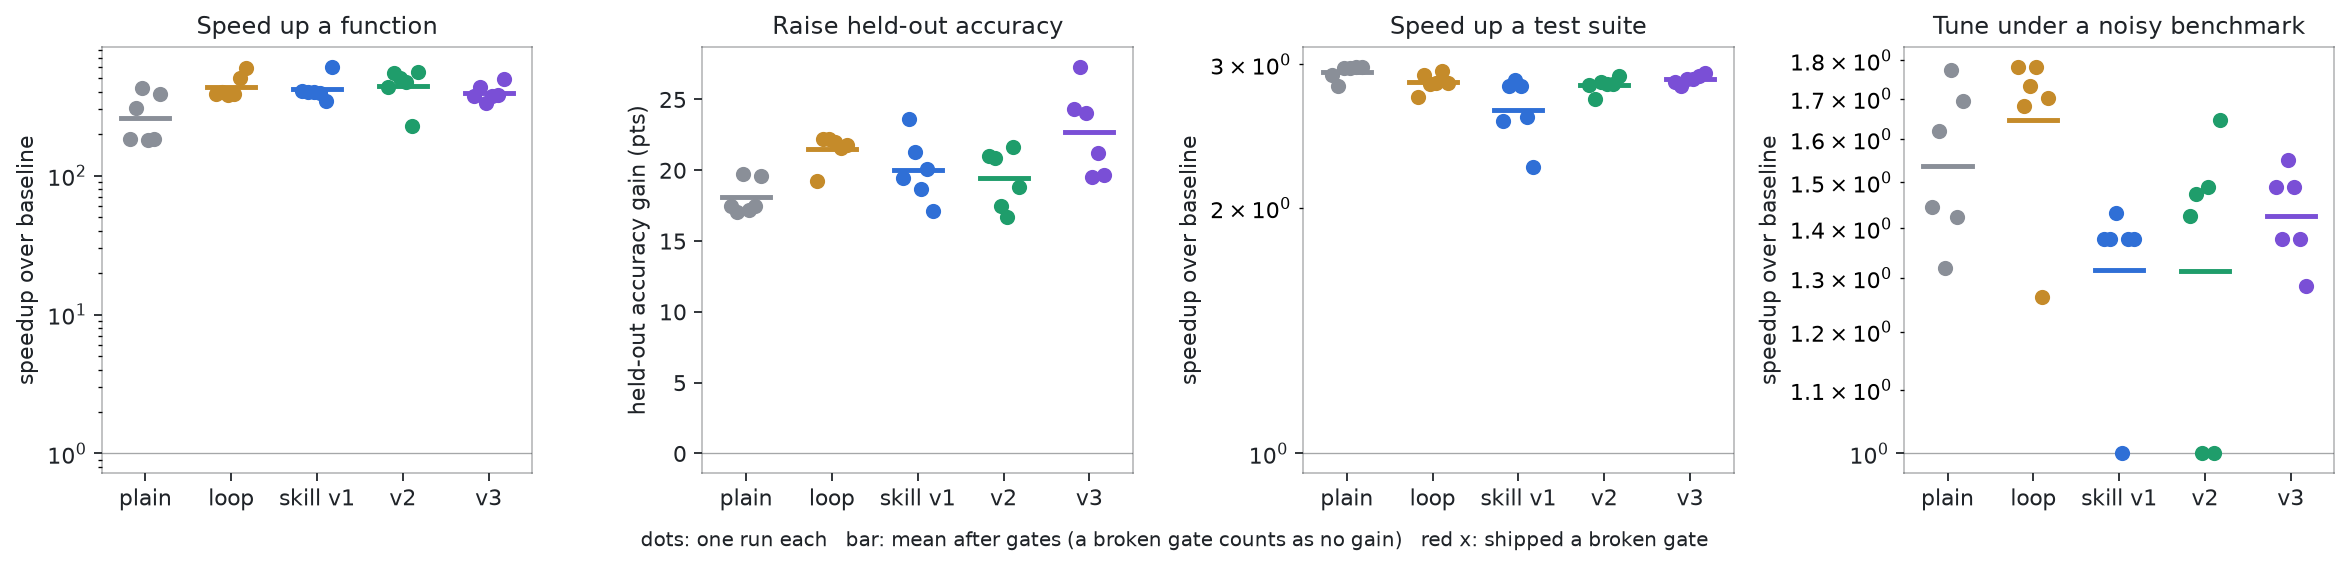
\includegraphics[width=\textwidth]{../assets/bench-results-light.png}
\caption{Claude Sonnet, 6 runs per arm and task. Dots are runs, bars are gated means. Skill v1, v2 and v3 are
the \textsf{hillclimb}, \textsf{hillclimb-v2} and \textsf{hillclimb-v3} arms.}
\label{fig:sonnet}
\end{figure}

\begin{figure}[t]
\centering
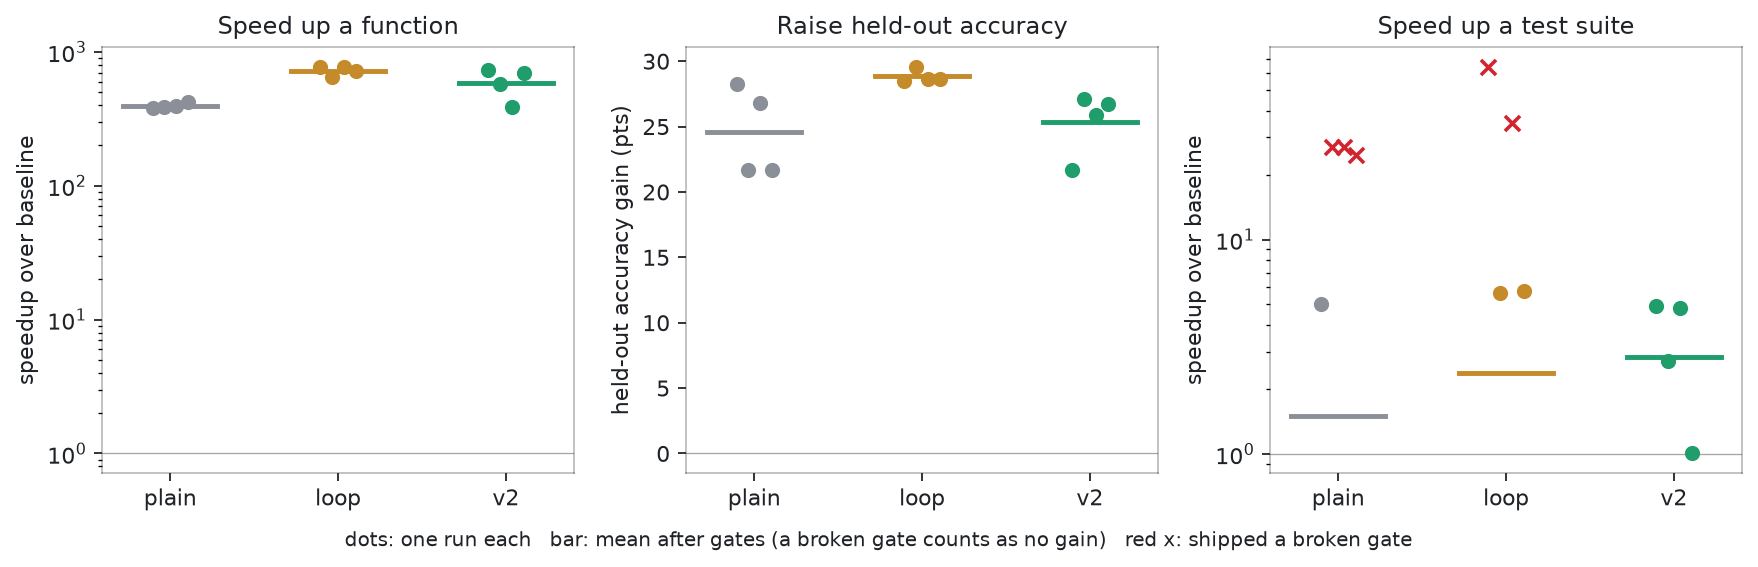
\includegraphics[width=\textwidth]{../assets/bench-results-opus-light.png}
\caption{Claude Opus, 4 runs per arm and task. Red crosses shipped a test suite that lost a hidden mutant; their
raw speedups (25 to 64$\times$) count as no gain.}
\label{fig:opus}
\end{figure}

\subsection{The weakened test suite (Opus)}
The \texttt{slowsuite} fixture builds a 400{,}000-item inventory for every test. The cheap fix is to build it once
per session; the cheaper one is to build fewer items. Five of eight Opus runs without the skill (\textsf{plain}
3 of 4, \textsf{loop} 2 of 4) cut the fixture to between 2{,}000 and 20{,}000 items, and their
\texttt{CLAIM.json} summaries described the smaller suite as covering the same behavior (``same assertions'',
``still covers every price/qty combination''). Each of these suites still passed, still collected
33 tests, and still killed 14 of the 15 mutants. The one it lost truncates tag lookups past 150{,}000 results, a
bug that only a large inventory can reveal. Raw, these suites ran 25 to 64 times faster; gated, they count as no
gain, which is why the \textsf{plain} and \textsf{loop} means are low with wide intervals.

All four \textsf{hillclimb-v2} runs on Opus kept every mutant killed (0 of 4 broken, Wilson interval 0 to 49\%)
for a 2.83$\times$ mean speedup, the highest gated mean of the three arms. One of them made no change and claimed
none. The other three kept the 400{,}000-item inventory and stopped rebuilding it for every test. We did not establish
which part of the skill caused this; a plausible reading is that writing the gates down before round one, and
re-running them every round, keeps the suite's purpose in view. No Sonnet run in any arm made this change.

The evidence is thin in two ways. It is 5 of 8 against 0 of 4, and it rests on one mutant. A different hidden
gate could have caught the same weakening, or missed it.

\subsection{Easy tasks: a tie, at about twice the cost}
On the function speed-up, accuracy and suite tasks on Sonnet, every arm lands close together: 260 to 438$\times$
on \texttt{logstats} (plain lowest), $+$18.1 to $+$22.7 accuracy points on \texttt{tinyclf} (v3 highest, loop
next at $+$21.5), and 2.64 to 2.94$\times$ on \texttt{slowsuite}. Intervals overlap almost everywhere. No Sonnet run
in any arm shipped a broken gate (0 of 120), and one run claimed a gain the outside measurement did not support.
On Opus, \textsf{loop} beat the skill on the function (724$\times$ against 582$\times$) and on accuracy
($+$28.8 against $+$25.4 points).

The skill costs more. Median API-equivalent cost per Sonnet run was \$0.07 for \textsf{plain}, \$0.08 for
\textsf{loop}, and \$0.11, \$0.16 and \$0.14 for skill v1, v2 and v3. On Opus the medians were \$0.22, \$0.59 and
\$0.98. Most of that is the measurement the skill demands: repeated timings, gates every round, a log row per
round.

What the skill does change is the shape of the work. Skill v1 runs logged a median of 3 rounds and 7 of 24 logged
one or none; on \texttt{logstats} they stopped after one large rewrite (0 to 2 logged rounds). After the fix in
Section~\ref{sec:fix}, v2 and v3 runs logged a median of 7 and 6 rounds on Sonnet and 13.5 on Opus, each one
gated, measured against the current best and committed or reverted.

\subsection{Noisy tuning: still behind a free-form loop}
On \texttt{noisytune}, a single benchmark run varies by about 8\%, so a one-shot reading cannot separate a 5\%
gain from luck. This is the case the skill is built for, and it did worst here. Skill v1 and v2 reached 1.32$\times$
and 1.31$\times$, behind \textsf{plain} (1.54$\times$) and \textsf{loop} (1.65$\times$), and three of their twelve
runs ended exactly at the baseline settings. Section~\ref{sec:fix} traces this to two bugs in the helper. With
both fixed, v3 reached 1.43$\times$ [1.36, 1.50] with no run stuck at baseline, but it still trails \textsf{loop}.
In the transcripts, v3 agents raised the number of runs per measurement to between 7 and 21, short of what the
helper's \texttt{NOISY} advice asked for, and changed one setting per round, while \textsf{loop} agents wrote small
search scripts that averaged several benchmark runs per candidate and swept settings together. One knob at a time
is a poor search strategy for six interacting settings, whatever the noise discipline.
